\documentclass{article}
\usepackage[utf8]{inputenc}

%---------------------------------------------------
%
%---------------------------------------------------

\usepackage{amsmath}
\usepackage{amssymb}
\usepackage{blindtext}
\usepackage{bm}
\usepackage{float}
\usepackage[margin=.75in]{geometry}
\usepackage{graphicx}
\usepackage{mathrsfs}
\usepackage{multicol}

\def\changemargin#1#2{\list{}{\rightmargin#2\leftmargin#1}\item[]}
\let\endchangemargin=\endlist

\renewenvironment{abstract}
{
\begin{changemargin}{0.5in}{0.5in}
}
{
\end{changemargin}
}

\newcounter{theorems}
\newenvironment{theorem}
{
\stepcounter{theorems}
\begin{changemargin}{0.25in}{0.25in}
\noindent
\textbf{Theorem \arabic{theorems}:}
\begin{em}
}
{
\end{em}
\end{changemargin}
}


\newenvironment{proof}
{
\begin{changemargin}{0.25in}{0.25in}
\noindent
\textbf{Proof: }
}
{
\begin{flushright}
$\blacksquare$
\end{flushright}
\end{changemargin}
}

%---------------------------------------------------
%
%---------------------------------------------------

\title{Run AwAI: StarCraftII Adversary Avoidance Using Neural Networks and
  Genetic Algorithms}

\author{Kyle R. Chickering \\ krchicke@ucdavis.edu
  \and Alex R. Mirov \\ armirov@ucdavis.edu
  \and Simon H. Wu \\ simwu@ucdavis.edu
  \and Xin Jin \\ jin@ucdavis.edu}

\date{June 8, 2018}

%% TODO: Why our approach vs other approaches
%% TODO: Random action is a fairly robust approach to the problem space
%% TODO: Include convergence Graphs in the results section
%% TODO: Talk about the mutation rates in the genetic algorithm
%% TODO: Reference the fact that neuro evolution is good in high dimensional
%%    and continuous state spaces (ref neat paper)

\begin{document}

\maketitle
\hline
\\~\\

\begin{abstract}
  \textbf{Abstract}: \blindtext
  \\~\\
  \textbf{Keywords}: Machine Learning, Genetic Algorithms, Neural Networks,
  StarCraftII
\end{abstract}
\\~\\
\hline
\\~\\

\begin{multicols}{2}
\section{Introduction}
Since AlphaGo's defeat of the Go champion Ke Jie, the artificial intelligence
community has
been looking for a new problem domain to apply learning techniques to. A
surprising candidate for artificial intelligence testing has
emerged in the form of real time strategy games. Real time strategy games work
by having a player make critical decisions in real time against an enemy
player. The game StarCraftII, released by Blizzard entertainment in 2010, is a
real time strategy
game that has captured the interest of the artificial intelligence community.
The game presents several challenges for artificial intelligence, the biggest of
which is the magnitude of possible game states. The game technically has a
finite number of game states, but the granularity of those states renders the
game practically continuous.

We present a method of teaching an agent to avoid enemy players for as long as
possibly by using genetic algorithms to evolve neural networks (neuroevolution).
We interface our neural network agents using the PySC2 library and evolve an
agent that shows a measurable increase in its ability to run away from
adversarial opponents.

\section{Background}
This project combines two proven artificial intelligence paradigms, neural
networks and genetic algorithms. These methods are traditionally orthogonal,
but there has been a growing body of work in recent years with regards to
evolving neural networks using genetic algorithms, most notably \cite{NEAT}.

\subsection{Neural Networks}
Neural networks are a method of computing any computable function by using a
network of nodes called \textbf{neurons} connected by a series of edges. This
representation is inspired by the human brain, and has been proven over and over
as a heavy hitter in the world of machine learning. These networks are
differentiable, and by calculating error, they can be trained using a method
called backpropogation that changes the strength of the connections between
neurons. The backpropogation method is the status quo of training neural
networks, however, alternative methods exist, such as neuroevolution.
Neuroevolution is an efficient alternative, especially in spaces with
continuous state spaces.

There are two main ways to represent neural networks in software, implicitly and
explicitly. Implicit neural networks use linear algebra and a consistent layered
structure to propagate inputs forward (called feeding forward). With numerical
linear algebra libraries available for almost every major programming language,
this method of representing neural networks allows for incredibly fast
processing
of neural networks. However, this representation's greatest strength, its speed,
is the source of its greatest weakness. Implicitly defined neural networks
suffer
from the inflexibility of their layered structure. In the human brain, neurons
are not limited to any specific structure, and are free to make connections
that could not be possible in a layered model.

This leads us to explicitly defined neural networks. These networks allow the
specification of new nodes that are disconnected from the traditional layered
model. While this can be advantageous, it can also present problems for the
implementer. Because these models are represented by graphs, we can no longer
use linear algebra libraries to feed forward through the network. This causes
an increase (often significant) in running time. For small networks this is
not an issue, but for larger network this becomes (sometimes prohibitively)
problematic.

\subsection{Genetic Algorithms}
In a similar line of though that led researchers to build neural networks by
looking to nature for inspiration, genetic algorithms exploit natural selection
to create optimal solutions to problems. Research into genetic algorithms
started when researchers realized that there is nothing inherent in evolution
that limits the process to nature \cite{dejong}. In fact, by thinking of
evolution as an algorithm in and of itself, we can extend the principles of
evolution to
digital systems. This is commonly done by defining what an "individual" and
"fitness function" mean in the digital evolution landscape. The algorithm
proceeds as evolution does in nature by picking the most well adapted
individuals to "breed", and evaluating their "offspring" on the same problem.
This technique has yielded several fascinating results, and often the
algorithm generates novel solutions to difficult problems \cite{lehman}.

\section{Methodology}
Our approach involves combining genetic algorithms and neural networks to
create an agent that learns through evolution how to evade antagonistic
agents. We chose this method as the problem space closely resembles nature's
predator/prey motif, and with such a large state space, neuroevolution is
actually an efficient solution \cite{NEAT}. By modeling our agent as an
evolving neural network we can
get results that mimic generational evolution in nature. While evasion,
especially in the StarCraftII space, is a fairly simple behavior, we chose this
method as it is easily extendable to larger problem spaces by extending the
input and output dimensions.

There are many techniques to accomplish running away from enemies in
StarCraftII, for example, a simple expert system would be quite good at enemy
avoidance, however we were concerned with the scalability of our approach. We
chose the neural network and genetic algorithm approach because for dealing
with more complex tasks, our approach is more robust than a simple expert
system. Additionally, we could train various neural networks on different
tasks (avoidance, attacking, resource mining, etc.) and splice the neural
networks together to build an AI capable of multitasking during the game.

By introducing scalability, we could use our existing framework to train neural
networks in more and more difficult simulated environments, eventually leading
to an AI that could play the entire game outside of a sandbox mode. Neural
networks generalize very well to a wide array of situations that are similar or
close to the situations they were trained on, and they are a perfect tool for
attacking a game that requires real time decision making and reasoning over a
complex set of inputs.

\subsection{Simulations}
To compute the fitness for each neural network in the population, we run the
network through a simulation. The simulation is run in StarCraftII, and our
simulation controller is built on top of the PySCII interface, and simulates
a ``game'' between our agent and a group of adversaries, which are controlled by
the in-game AI that ships with the game.

Each simulation is called an episode, and we ran the networks through 5-10
episodes each so that we could get a representative sample of the amount of time
that each neural network was able to survive.

We let the neural network choose the next action from our action space, which
consists of a series of movement directions (eight cardinals and a stay
command). The game runs a ``continuous'' time simulation (obviously continuity
is limited by the computer's capabilities), but we chose to have our neural
network make decisions in finite time intervals. We did this so that we would
not fall victim to our network not making decisions fast enough, and chose a
time step that would allow the network to make decisions quickly enough to
function well.

\begin{figure}[H]
\centering
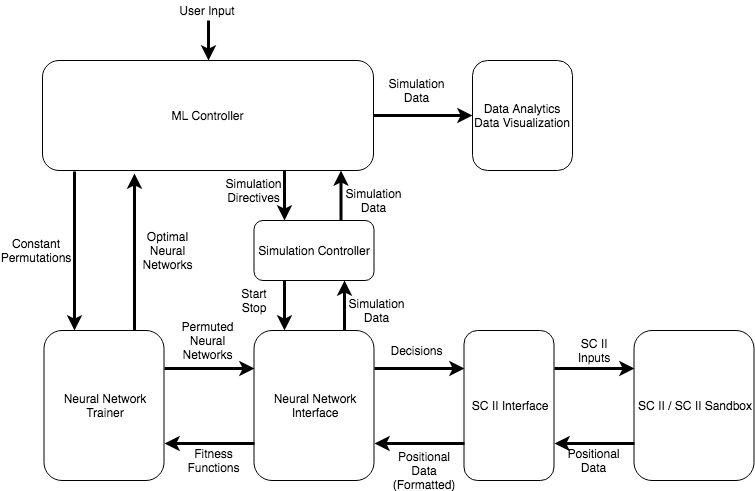
\includegraphics[width=0.45\textwidth]{chart}\label{fig:flow chart}
\begin{changemargin}{0.15in}{0.15in}
  \caption{Control and data flow through the Run AwAI controller.}
\end{changemargin}
\end{figure}

Our whole system ran as outlined in \ref{fig:flow chart}. We decoupled the
various aspects of the system as outlined as a good architecture practice in
\cite{pragprog}. We run a general simulation controller, which interfaces with
the neural networks through a module, and after creating and manipulating the
networks, sends them to a simulation controller which interfaces with PySC2,
which runs the simulations in StarCraftII.

We collect from each simulation the set $\bm{\mathcal{E}}$ of episodes, which we
can use to collect data from the simulation. We also compute the number of steps
taken by our agent in each simulation, denoted
$\mathcal{S}(e\in\bm{\mathcal{E}})$. The steps are the number of actions that
the agent made during the simulation, and we chose to measure this because it is
a good indicator of success of the agent at running away.

\subsection{Neural Network}
We started by using an explicit neural network implementation, which we chose
because we were curious if the flexible topologies would lead to a more
efficient neural network. We were inspired by the NEAT algorithm \cite{NEAT}, which has
shown promise in other video game domains. However we choose a simpler
topologically explicit implementation to simplify and accelerate the development
of our
algorithm. We ultimately settled on an acyclic graph representation, which
allowed us the freedom to add nodes and allowed simple manipulation of
connection weights.

We chose to use our neural network to represent a function taking an input
vector $\bm{I}$ consisting of relative agent position and adversary's relative
position and return an output vector $\bm{V}$ of floating point values
corresponding to the agent's belief that a particular action would lead to a
successful outcome. The neural network is a function
$\mathcal{N}:\text{dim}(\bm{I})\rightarrow\text{dim}(\bm{V})$:
\begin{align}
  \bm{V} = \mathcal{N}(\bm{I})
\end{align}
We choose the next action according to the simple maximization equation:
\begin{align}
  a_n = \max_{v \in \bm{V}} \: v
\end{align}
This input vector is flexible, and allows us to tweak the information that we
feed to the neural network. Additionally, while the output space we used
contains only movement in the cardinal directions, we could easily add other
supported actions like attacking and mining resources.

Our neural network uses the standard sigmoid function $\varsigma$ as its
activation function:
\begin{align*}
  \varsigma(x) = \frac{1}{1 + e^{-x}}
\end{align*}
We chose this function for a number of reasons, the least of which is its
popularity as an activation function in neural networks. Because of the shape of
the sigmoid function, inputs to subsequent neurons stay in the nice range of
$[-1, 1]$, which has the effect of normalizing the network. Since we are not
using backpropogation, the nice properties of the sigmoid function were
unimportant to us. However, if we were to do live backpropogation during
simulations (See section \ref{sec:improvements}), the sigmoid function would be
a useful activation function.

When we initialize the network, we populate all of the connection weights from a
random Gaussian distribution with $\sigma = 1$ and $\mu = 0$. This serves to
make our input data ``nice'' for the sigmoid function, which ends up returning
either $1$ or $-1$ when the input data is amplified by non-gaussian data. This
also ensures that most connections are ``off'' or close to off at the start,
which allows the network to learn without any random pre-bias. Our first
generation will have very weak suggestions on the effectiveness of the next
move. This may seem counter-productive, but it allows us to do much slower
mutation changes to the connection weights, which in turn increases the
explorative power of our algorithm at the start of the evolutions. If the
weights are too heavy in the beginning, the agent will favor a local maximum
almost immediately, but with a Gaussian distribution, the algorithm explores
more options before settling on a specific maximum.

\subsection{Genetic Algorithm}
For our implementation, we used a tournament style selection process to choose
our most fit individuals. We use tournament selection over other selection
methods (like probabilisitic selection), to improve convergence speeds.
Tournament selection is an exploitive selection method, and we choose exploitive
behavior over exploratory behavior because our simulation was a substantial
bottleneck in our iterative process. Because we choose an exploitive method, we
limit the chances of finding a global maximum, but increase the chances of
finding some local maximum, and finding it relatively quickly. This gave us a
chance to better observe the convergence of our algorithm, and allowed us to
demonstrate clear forward progress.

To get convergence, we spent a lot of time looking at fitness functions. We
considered many different possibilities, but finally settled on a measure of the
number of steps that our agent took during the simulation, with a penalty for
inconsistency. We figured that this would be a good measure of our agent's
ability to stay alive, and we thought that time alive was a good indicator of
the agent's ability to accomplish the goal of running away. We computed the
fitness $F$ using the following formula:
\begin{align}\label{eq:fitness}
  F(\bm{i}) = \frac{1}{|\bm{\mathcal{E}}|} \sum_{e
\in \bm{\mathcal{E}}} \mathcal{S}(e) - \eta\sqrt{\frac{1}{|\bm{\mathcal{E}}|}
\sum_{e \in \bm{\mathcal{E}}}\left(\mathcal{S}(e) - \frac{1}{|\bm{\mathcal{E}}|}
\sum_{e \in \bm{\mathcal{E}}} \mathcal{S}(e)\right)^2}
\end{align}
where $\bm{\mathcal{E}}$ is the set of all episodes run by the PySC2
simulation, $\mathcal{S}(e)$ is the number of steps taken by the agent in the
episode, and $\bm{i}$ is a an individual of the population. $\eta$ is a
hyper-parameter we use to fine tune the convergence of our network. We are
effectively calculating the average number of steps and penalizing the
individuals based on the standard deviation from the mean of the episodes. This
penalty serves to mitigate the effects presented by individuals that get
``lucky'' and have a few good trial runs that offset their average.

We seed the evolutionary controller using $n$ random individuals, and in each
evolutionary iteration, we breed $n\text{C}2$ individuals to compose the
subsequent generation. After breeding, we randomly mutate some of the children,
and then calculate the fitness for each individual in the population. To get the
next generation, we choose the most fit $n$ individuals from the population to
breed, and repeat the cycle. In addition, we found that the algorithm converged
more rapidly if we let the most fit individuals survive to the next generation,
and after making this change we noticed a jump in convergence rates.

The genetic algorithm relies on several hyper-parameters. The most obvious is
the population size. We find, unsurprisingly, that larger population sizes are
more robust and promote faster convergence, this makes intuitive sense because
with larger population sizes there is an increased chance of mutation, and
mutations are largely responsible for exploratory behavior in learning
algorithms. We have three mutation parameters, which are the rate at which nodes
are added to the network, the rate at which new connections are added to the
network, and the rate at which connection weights are changed.

We mutate connection rates based on a Gaussian distribution, which, combined
with our Gaussian weight initialization, ensures that weights never change
dramatically. We adjust weights according to the formula:
\begin{align}
  w_i \leftarrow w_i + \bm{\sigma}
\end{align}
where $\bm{\sigma}$ is a random variable from a Gaussian
distribution. We found that changing the weights according to a Gaussian
distribution promoted faster convergence than using weights taken from a uniform
distribution.

\subsection{Controller}

\subsection{PySC2 Interface}
Our simulation learning environment was based on an existing environment
included in the PySC2 library\cite{pysc2}. We use the ``Defeat Roaches'' mini
game as the baseline for our learning. Once we had the map, we used the
StarCraftII map editor to tweak the mini game to better suit our needs. We
created three maps that were used in testing. The default map is a simple square
map which spawns a group of adversarial ``roaches'', and a group of ``marines'',
who are controlled by our agent. The marines and roaches are spawned in the same
place every time, which gives us a consistent platform to test our agent.

The second variation is similar to the first, except that there is only one
``roach'' and one ``marine''. This map type highlights the capabilities of our
agent in a more intimate setting. The group of marines has the advantage of
being able to get ``lucky'' and have some members survive, but the one-on-one
variation forces the neural network to work well from the very beginning.  With
the one-on-one map, we were hoping to highlight more explicitly the capabilities
of our trained neural networks.

The third map variation was a larger sized version of the original map, which we
made in the hopes that we would see different convergence rates and survival
strategies on a larger game space. We were hoping to see the agent take
advantage of the larger space, but unfortunately did not have time to run
extensive simulations on this map.

All three maps have a slight bit of non-determinism built in, which means
subsequent simulations using the same neural network will not be identical. This
gave us the opportunity to gather more realistic data about the performance of
our agent, since we could accumulate an average over a number or trials.

\section{Results} We ran several simulations with various choices of
hyper-parameters, and our results were promising. We saw measurable improvement
in performance after just a few iterations of the algorithm, which gave us a
steep initial learning curve before the improvements started to taper off.

\begin{figure}[H]\label{fig:fitness graph}
\centering
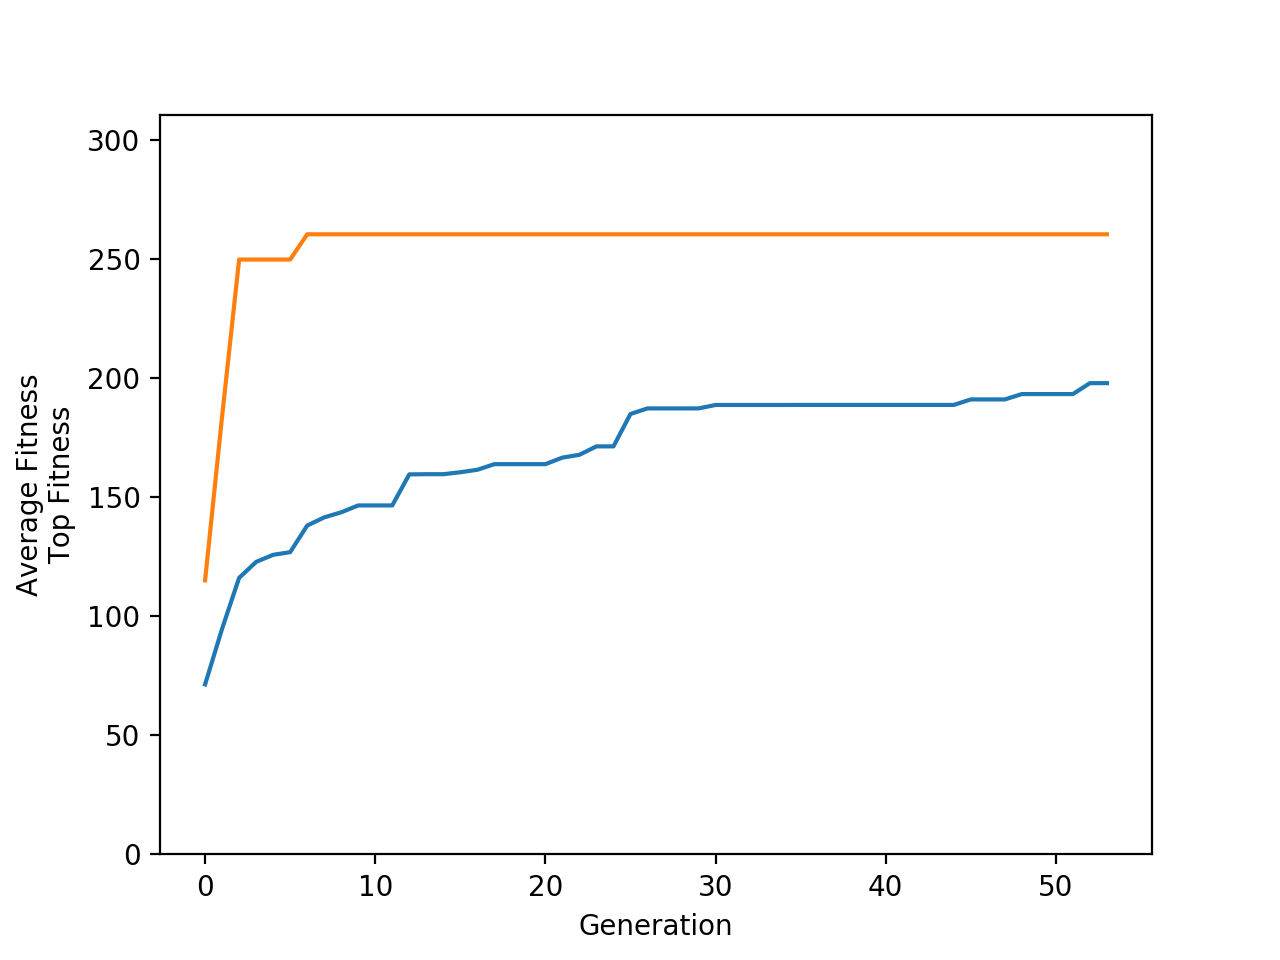
\includegraphics[width=0.45\textwidth]{fig_1}
\begin{changemargin}{0.15in}{0.15in}
  \caption{Graph of average fitness (blue) and top fitness (orange) for each
    generation in Trial 1. Top fitness is the fitness of the most fit individual
    at the end of each generation's simulations. Average fitness is calculated
    by averaging \eqref{eq:fitness} over all individuals $\bm{i}$ in the
    population. The breeding constant is set to 15, node generation rate is set
    to 0.3, new connections at 0.2 and non structural mutations at a rate of
    0.4}
\end{changemargin}
\end{figure}

We see in Figure \ref{fig:fitness graph} an artifact from our choice of genetic
algorithm. Because we keep the top individual from each generation in the gene
pool, we see that the top individual has plateaued early, and no new individual
is achieving a higher fitness. We see that the average is continually increasing
though, which will increase the chances that an individual will eventually be
bred that has a higher fitness than the individual that is dominating the
maximum fitness.

We can also see that the average sometimes plateaus as well. This is due to a
homogenization of the gene pool, where the children individuals are very
similar to their parents. Because of low mutation rates in this trial, we got
``unlucky'' and were not creating enough mutations to be exploratory, this is a
case of finding a local maximum. Since we favored an exploitive algorithm, this
is to be expected, however we see that the population can still achieve higher
fitness measures which means that the algorithm still retains some amount of
exploratory behavior.

\begin{figure}[H]\label{fig:fitness graph}
\centering
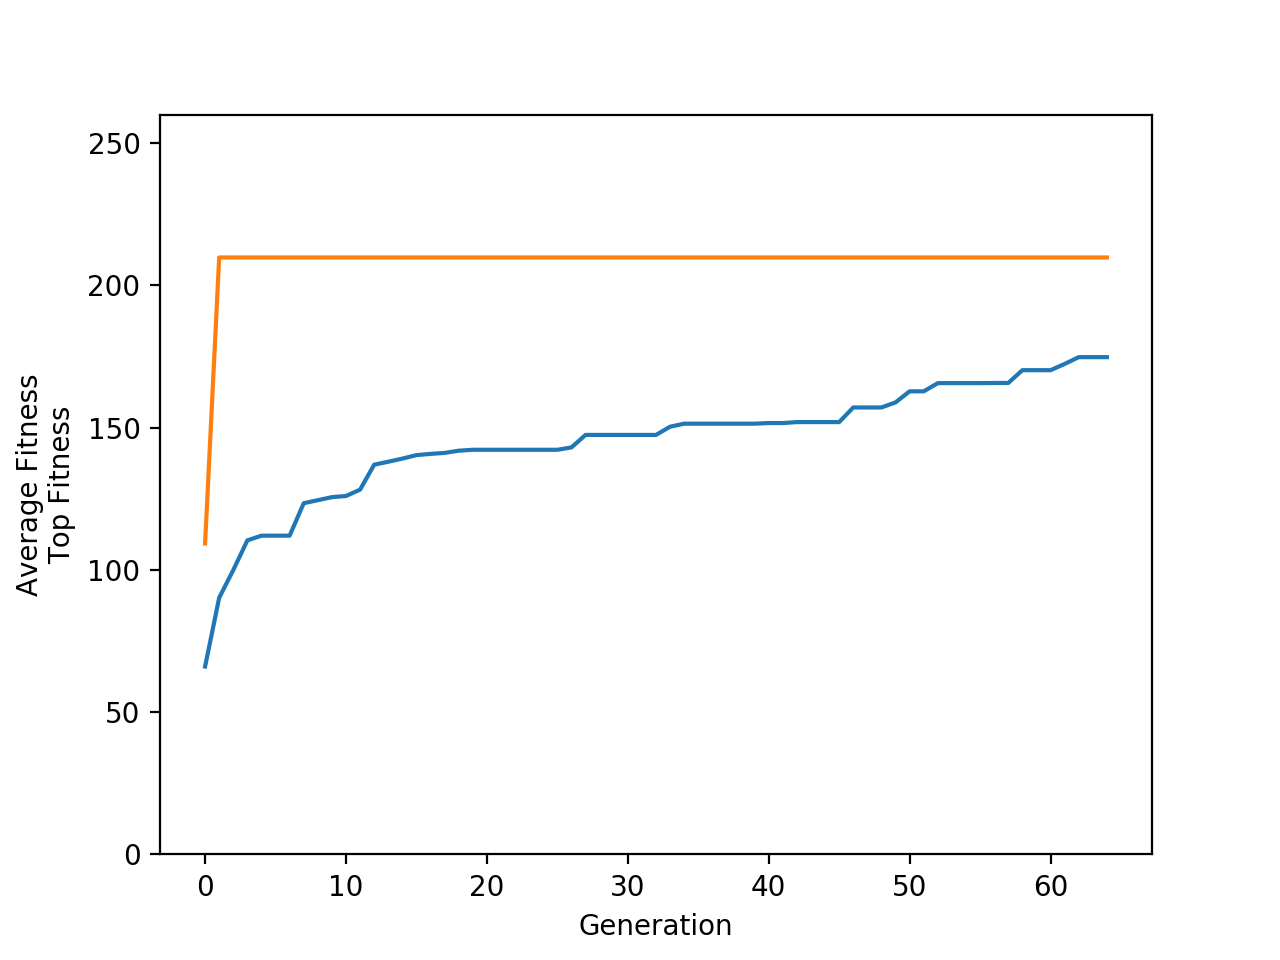
\includegraphics[width=0.45\textwidth]{fig_2}
\begin{changemargin}{0.15in}{0.15in}
  \caption{Graph of average fitness (blue) and top fitness (orange) for each
    generation in Trial 1. Top fitness is the fitness of the most fit individual
    at the end of each generation's simulations. Average fitness is calculated
    by averaging \eqref{eq:fitness} over all individuals $\bm{i}$ in the
    population. The breeding constant is set to 15, node generation rate is set
    to 0.5, new connections at 0.5 and non structural mutations at a rate of
    0.75}
\end{changemargin}
\end{figure}

In our second trial, we see that the average fitness increases much more
regularly. However, despite having more generations, trial two did not reach the
same average fitness or top fitness as trial one did. One possible reason for
this behavior is that our mutation rates are higher, so our algorithm favored a
more exploratory approach, leading to a more consistent increase in
fitness. This exploratory behavior also accounts for the top fitness being lower
than in trial one.

We did not have enough time to run extensive testing over a representative
sample of hyper parameters, and expect to get better convergence by tweaking the
parameters some more. We chose the parameters we did so that we could see
convergence in a timely manner. Since our simulation times were the bottleneck
in our pipeline, we choose a relatively small population size to run through our
algorithm. We think that using higher population sizes would also lead to better
convergence, as the networks would be put through more and more simulations,
generating a more and more accurate picture of their fitness.

%% TODO: Talk about choice of hyper parameters, population size, episode count
%% mutation constants, eta in fitness function

\section{Conclusion}
Different selection types?
\blindtext

\subsection{Improvements}\label{sec:improvements}
% live back propagation
One of the for-most improvements we could do is to train the neural networks
during the simulation as well as training them through evolution. In addition
to improving the convergence, this strategy would mimic nature even more.
Organisms learn during their lifetimes, and there is speculation that the knowledge obtained by an individual during its lifetime can be passed down through the
genome.

We could accomplish this by using backpropogation during the simulations, and considering good measures of progress that we could calculate during the game. As an example, we could compute the Euclidean distance between the agent and the adversary and make decisions that minimize this value. The drawback to this method is that it may encourage sub-optimal behavior by biasing the agent towards known behavior. It is common for human experimenters to expect sub-optimal behavior because optimal behavior is so far unknown \cite{lehman}.

\subsection{Future Work}
This project can certainly be extended in many ways, for example, we could
extend the output vectors to include offensive maneuvering by our agent, and
train the agent to be aggressive by considering the number of adversaries killed
by our agent during the simulation.

Another possibility that we did not explore, was the effect of removing neurons
from the network. Neural networks can often be plagued by overfitting input
data, and by removing neurons we hypothesize that any overfitting we encounter
could be mitigated. We would remove these neurons in the same way that we add
neurons, that is, non-deterministically as a possible mutation. In the study of
biological creatures, we often see either total dropping of traits from the
population genome or the transition to vestigial genetic structure
\cite{lehman}. In keeping with this, instead of outright removing the neuron, we
could significantly decrease the strength of the connections to it, essentially
removing it from the network. If the neuron in question was indeed problematic,
we would see it continue to evolve very low weights, essentially pruning the
neuron and rendering it vestigial.

We could also track the lifespan of certain individuals and kill them off after
a certain number of generations. We found that the algorithm would sometimes
plateau with a very fit individual for a period of time, and it would be
interesting to see what effects a notion of ``lifetime'' would have on the
algorithm as a whole.

\end{multicols}

\\~\\
\hline
\\~\\

\begin{thebibliography}{9}
\bibitem{NEAT} 
  Kenneth O. Stanley, Risto Miikkulainen.
  \textit{Evolving Neural Networks through Augmenting Topologies}. 
  The MIT Press Journals.

\bibitem{dejong}
  Kenneth A. De Jong. \textit{Evolutionary Computation: A Unified Approach}.
  MIT Press, Feb 3, 2006.

\bibitem{russell}
  Stuart Russell, Peter Norvig.
  \textit{Artificial Intelligence: A Modern Approach}.
  Upper Saddle River (New Jersey, 1995).

\bibitem{lehman}
  Joel Lehman et al.
  \textit{The Surprising Creativity of Digital Evolution: A Collection of
    Anecdotes from the Evolutionary Computation and Artificial Life Research
    Communities}.
  \textbf{https://arxiv.org/pdf/1803.03453.pdf}.

\bibitem{pysc2}
  Google DeepMind pysc2.
  \textbf{https://github.com/deepmind/pysc2}.

\bibitem{pragprog}
  Andrew Hunt, David Thomas.
  \textit{The Pragmatic Programmer: From Journeyman to Master}
  Addison-Wesley (Reading, Mass., 2000)

\end{thebibliography}

\end{document}